\documentclass[pdftex,bibtotocnumbered,idxtotoc,twoside]{scrartcl}
\usepackage[T1]{fontenc}
\usepackage[utf8]{inputenc}

\usepackage{amsfonts}
%\usepackage{lmodern}
\usepackage{graphicx,wrapfig}
\usepackage{url,acronyms,myref}
\usepackage{listings}
\usepackage{lstomdoc}
\usepackage{xmlindex}
\usepackage{tikz}
\usepackage[show]{ed}
\usepackage[margin={2.5cm,2.5cm,1.5cm,1.5cm}]{geometry}
\usepackage[fancyhdr,today,draft]{svninfo}
%\usepackage{hyperref}% Load this last!
\pagestyle{fancyplain}\fancyhead[RE,LO]{\leftmark}\fancyhead[LE,RO]{\thepage}
\def\javascript{{\sc{JavaScript}}}
\def\llquote#1{\ensuremath{\langle\kern-.25em\langle\hbox{\sl{#1}}\rangle\kern-.25em\rangle}}
\def\mod{{\rm{mod}}}
\def\pres#1#2{\overline{#1}^{#2}}  
\def\lden{[\kern-.15em[}\def\rden{]\kern-.15em]}
\def\defemph#1{{\bf{#1}}}
\def\imarg#1#2{\fbox{\ensuremath{\left.#1\right|_{#2}}}}
\def\fimarg#1#2#3{\fbox{\ensuremath{\left.#1\right|_{#2}^{#3}}}}
\def\recu#1{#1}%should be changed to notation for <recurse precedence="#1"/>, maybe a circle around p
\lstset{float=htb,columns=flexible,frame=lines,language=[omdoc]XML,basicstyle=\scriptsize,
        indexstyle=\indextt,indexstyle=[1]\indexelement,indexstyle=[2]\indexattribute,
        numbers=left,stepnumber=5,numberstyle=\tiny,showstringspaces=false}

\newcommand{\PC}{\mathcal{PC}}

\def\name#1{{{\small{\sc{#1}}}}}

\title{Presenting Mathematical Content With Flexible Elisions}
\author{Michael Kohlhase, Christoph Lange, Florian Rabe\\ 
  Computer Science, Jacobs University Bremen\\
  D-28759 Bremen, Germany \\ 
  \url{http://kwarc.info}}
 %\url{<m|c|f|n|ch|a|i>.<lastname>}@jacobs-university.de}
%m.kohlhase/c.mueller/f.rabe/n.mueller/ch.lange/a.kohlhase/i.normann

\begin{document}
\svnInfo $Id: presel.tex 7030 2007-10-17 12:47:55Z frabe $
\svnKeyword $HeadURL:https://svn.omdoc.org/repos/omdoc/branches/omdoc-1.2/projects/omdoc-2.0/OpenMath-paper/presel.tex
$
\maketitle
\begin{abstract}
  Mathematicians frequently elide brackets or symbols in formulae to concentrate on
  essential facts and to avoid distracting experienced mathematicians with notation that
  can easily be deduced from context. In this paper we propose a extension of the notation
  specification infrastructure in {\omdoc} by functionality for flexible elisions.
\end{abstract}
\tableofcontents

\svnInfo $Id: intro.tex 6561 2007-06-24 06:30:57Z kohlhase $
\svnKeyword $HeadURL: https://svn.omdoc.org/repos/omdoc/projects/omdoc-2.0/OpenMath-paper/intro.tex $
\section{Introduction}\label{sec:intro} 

Over the last three millennia, mathematics has developed a complicated two-dimensional
format for communicating formulae (see e.\,g.~\cite{Cajori:ahmn93,Wolfram:mnpf00} for
details). Changes in notation have been influential in shaping the way we calculate and
think about mathematical concepts, and understanding mathematical notations is an
essential part of any mathematics education.

Content Markup formats for mathematics such as {\openmath}~\cite{BusCapCar:2oms04} and
{\mathml}~\cite{CarIon:MathML03} concentrate on the functional structure of mathematical
formulae, thus allowing mathematical software systems to exchange mathematical
objects. For communication with humans, these formats rely on a ``presentation process''
(usually based on XSLT style sheets) that transforms the content objects into the usual
two-dimensional form used in mathematical books and articles.

After a conceptual analysis of the presentation process and a survey of recent approaches
to specify the notations of mathematical symbols and how to use these specifications to
transform content-oriented mathematical documents to a presentation-oriented format like
PDF or HTML, we introduce a revised specification of the presentation module of {\omdoc}
that is enabled for elisions.  We conclude by proposing how information about elisions
that a presentation algorithm performed can be included in the presentation markup and
used by a client application.

\subsection{Presentation as Composition and Elision}

Many such presentation processes have been proposed, and all have their strengths and
weaknesses. In this paper, we conceptualize the presentation of mathematical formulae as
consisting of two components: the two-dimensional {\defemph{composition}} of visual
sub-presentations to larger ones and the {\defemph{elision}} of formula parts that can be
deduced from context.

Most current presentation processes concentrate on the relatively well-understood
composition aspect and implement only rather simple bracket elision algorithms. But the
visual renderings of formulae in mathematical practice are not simple direct compositions
of the concepts involved: mathematicians gloss over parts of the formulae, e.\,g.\ leaving
out arguments, iff they are non-essential, conventionalized or can be deduced from the
context. Indeed this is part of what makes mathematics so hard to read for beginners, but
also what makes mathematical language so efficient for the initiates. A common example is
the use of $\log(x)$ or even $\log x$ for $\log_{10}(x)$ or similarly $\lden t\rden$ for
$\lden t\rden_{\cal M}^\phi$, if there is only one model $\cal M$ in the context and
$\phi$ is the most salient variable assignment. Another example are the bracket elision
rules in arithmetical expressions: $ax+y$ is actually $(ax)+y$, since multiplication
``binds stronger'' than addition. Note that we would not consider the ``invisible times''
operation as another elision, but as an alternative presentation. Finally, there are
extreme examples of elision or substitution like Church's dot notation, where a dot stands
for a left bracket, whose mate is as far to the right as consistent with the remaining
(un-elided) brackets. For instance $(a\cdot.\,b+c)-d$ stands for $(a\cdot(b+c))-d$, and
$\forall x,y.\phi\wedge\psi$ stands for $\forall x,y (\phi\wedge\psi)$.

Now that we have convinced ourselves that the elision is an important component of
generating high-quality presentations, let us reconsider the presentation process itself
to see how composition and elision interact.

We will start from the observation that in content markup formalisms for mathematics
formulae are represented as ``formula trees''. Concretely, we will concentrate on
{\openmath} objects, the conceptual data model of {\openmath} representations, since it is
sufficiently general, and work is currently under way to re-engineer content {\mathml}
representations based on this model. Furthermore, we observe that the target of the
presentation process is also a tree expression: a layout tree made of layout primitives
and glyphs, e.\,g.\ a presentation {\mathml} expression. If we make examples with
{\TeX/\LaTeX} it is only since it is universally understood; here, the layout tree is the
parse tree implicit in the linear {\TeX/\LaTeX} string. This notwithstanding, we finally
observe that even though formula presentations are two-dimensional in principle, large
parts are more or less linear, and therefore mathematical notation relies on brackets to
allow the reader to reconstruct the content structure from the presentation.

\subsection{Characteristics of Mathematical Symbols}\label{sec:characteristics}

In a nutshell, {\openmath} objects are trees built up from {\defemph{variables}} and
{\defemph{symbols}} at the leaves and {\defemph{applications}} and {\defemph{binders}} as internal
nodes. 

\begin{wrapfigure}{r}{3cm}\vspace*{-.5em}
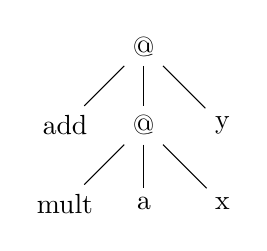
\begin{tikzpicture} 
\node (top) at (1,2) {@};
\node (plus) at (0,1) {add};
\node (mid) at (1,1) {@};
\node (y) at (2,1) {y};
\node (mult) at (0,0) {mult};
\node (a) at (1,0) {a};
\node (x) at (2,0) {x};
\draw(top) -- (plus);
\draw(top) -- (mid);
\draw(top) -- (y);
\draw(mid) -- (mult);
\draw(mid) -- (a);
\draw(mid) -- (x);
\end{tikzpicture}\vspace*{-.5em}
\end{wrapfigure}
For our purposes, symbols and applications are the most important concepts,
therefore let us fortify our intuition with the example on the right: the sum $ax+y$ above
would be represented by a tree with an application at the root, whose first child is the
symbol\footnote{Note that a symbol is not a glyph --- these are often confused, the symbol
  here stands for the mathematical concept of a sum, not the glyph $+$.} for addition, the
third child is the variable with the name $y$, and the second child is another application
whose children are the symbol for multiplication and the variables with names $a$ and $x$.

As part of the functional notation of mathematics popularized by Leibniz and Newton for
algebra, the visual appearance of a subformula was largely determined by its head
operator, which nowadays carries much of the notational conventions, which are usually
phrased in terms of the following notational characteristics of a symbol:

\begin{description}
\item[fixity (for operators):] Is the operator displayed as a prefix (like a function
  symbol), as a postfix (like the factorial symbol $!$) or as an infix (like most
  arithmetic operators)?  Operators of higher arity can also have a ``mixfix'' style;
  consider the 4-ary typing judgment operator $\Gamma\vdash_\Sigma t\colon\alpha$, which
  states that a term $t$ has type $\alpha$ in a variable context $\Gamma$ and a signature
  $\Sigma$.
\item[left and right brackets:] If an operation is bracketed, are round, square, curly,
  angle, or other brackets used? In fact brackets in mathematical vernacular are mostly
  round brackets; technical notations sometimes use others, e.g. {\mathematica} uses
  square ones throughout. Note that not all parts of a presentation that look like
  brackets are indeed. For instance in a half-open interval as $]a;b]$, is actually mixfix
  operator where the bracket-like glyphs ``$]$'' look and conventionally stretch like
  brackets, but do not match and cannot be elided like brackets. They are easy to mistake
  for brackets, since they (as all fully inhabited mixfix presentations) make brackets for
  the arguments unnecessary. We would consider it a semantic anomaly to present an
  ``interval'' operator as an infix ``;'' with obligatory left and right brackets ``$]$''
  and ``$]$''.
\item[precedence (for operators):] If an operation $O$ with a high precedence occurs as an
  argument of an operator with a lower precedence, the brackets around $O$ can be
  elided.
\item[associativity (for infix operators):] To elide brackets for $n$-ary operators
  ($n>2$), it must be known whether they are associative (i.\,e.\ $(a\circ b)\circ c =
  a\circ(b\circ c) =: a\circ b\circ c$) or obey ``left-associative'' or
  ``right-associative'' elision conventions (e.g.
  $\alpha\to\beta\to\gamma:=\alpha\to(\beta\to\gamma)$ for right-associative function
  types).
\end{description}
The first two characteristics specify the composition of the visual representations,
whereas the latter two are concerned with bracket elision. Furthermore, the {\bf{role}} of
a symbol in the formula context needs to be taken into account: Is it a simple
{\emph{constant}} like $\mathbb{R}$, a {\emph{function}} that is applied to arguments, or
a {\emph{binder}} that binds variables like $\forall x.p(x)$. This is most pronounced for
functions that can occur either applied to arguments or as the concept alone.
Presentations differ for these occasions, e.g. for the absolute value function, we write
something like $\bigl|\cdot\bigr|$ with a ``dummy argument'' $\cdot$ when it is not in an
applied context.

\subsection{Notation Definitions}\label{sec:notdef}

Mathematical formulae given in the XML-based structural formats {\openmath} and Content
{\mathml} are commonly presented by implementing one XSLT template~\cite{W3C:xslt2} per
symbol, which specifies how to transform this symbol to the output format---another XML
format like Presentation {\mathml}, or a non-XML format like {\TeX}, for example.
Appropriate templates for the arguments are usually applied recursively.

The following listing shows a straightforward way to transform the exponentiation operator
from {\openmath} to {\TeX}:
 
\begin{lstlisting}[language=XSLT,caption=An XSLT presentation template,label=lst:template]
 <xsl:template match="om:OMA[om:OMS[@cd='arith1' and @name='power']]">
   <xsl:apply-templates select="*[2]"/> <!-- first argument -->
   <xsl:text>^{</xsl:text>
   <xsl:apply-templates select="*[3]"/> <!-- second argument -->
   <xsl:text>}</xsl:text>
 </xsl:template>
\end{lstlisting}

To save authors from the tedious and error-prone task of writing similar templates for
every symbol and notation variant, different facilitations have been invented. The
probably earliest examples were the presentation architecture in
{\omdocv{1.0}}~\cite{Kohlhase:otormd00} and Naylor's\&Watt's {\openmath}
conversion~\cite{Naylor:conversion}. Both supply XML-based {\defemph{notation
    definitions}} that can be transformed into a suitable XSLT conversion style sheet by a
meta-stylesheet.

In {\omdoc}, a template like the one above would be generated from a
{\element{presentation}} element of the form
\begin{lstlisting}[mathescape]
<presentation for="power" theory="arith1" role="application" class="1">
  <style format="TeX">
    <recurse select="*[2]"/><text>^{</text><recurse select="*[3]"/><text>}</text>
  </style>
  $\ldots$
<presentation>
\end{lstlisting}
where the {\attribute[ns-elt=xsl]{match}{template}} attribute is generated from the
attributes on the {\element{presentation}} element and the contents from the ones on the
{\element{use}} element. In contrast to this, where notations definitions are thought as
directed rules from content to presentation, Naylor's\&Watt's framework views them as
equivalences between representations. For the example above we would have
\begin{lstlisting}[mathescape,language=XML,morekeywords={Notation,version,semantic-template},
caption=A Template-Based Notation Definition,label=lst:template-based]
<Notation>
  <version style="1">
    <tex>\arg{a1}{n}^{\arg{a2}{m}}</tex>
    $\ldots$
  </version>
  <semantic-template>
    <OMA><OMS cd="power" name="arith1"/>
      <OMV name="n" id="a1/>
      <OMV name="n" id="a2/>
    </OMA>
  </semantic-template>
</Notation>
\end{lstlisting}
We will call the first approach to notation specification {\defemph{symbol-based}}, as the
notation is tied to a concrete symbol, and the second one {\defemph{template-based}}. Note
that the template-based approach is in principle more directly invertible (e.g. for
parsing), and more expressive (it would e.g. allow to present $log(e,x)$ as $\ln(x)$ and
$log(b,x)$ as $\log_b(x)$). But this has not been realized in practice, since the
presentation of mathematical formulae {\emph{is indeed}} tied to symbols, so all templates
are indeed one-level like the one in the example above. On this fragment, both approaches
are equivalent. Note furthermore that many of the notational characteristics of a symbol
mentioned in section~\ref{sec:characteristics} actually do not belong to the symbol but to
its presentation. For example, the division operator, presented as $\cdot/\cdot$, has a
higher precedence than $\frac{\;\cdot\;}{\;\cdot\;}$---consider $1/(a+b)$ vs.\
$\frac{1}{a+b}$.

In {\omdocv{1.2}}~\cite{Kohlhase:omdoc1.2}, all of these characteristics can be specified
as attributes to one out of potentially multiple {\element{presentation}} elements that
refer to a {\element{symbol}}. For some aspects like mix-fixity, this declarative syntax
is not yet expressive enough; in this case, embedded XSLT templates must be used, losing
declarativity. In this paper, we rethink the notation definition system and propose a
declarative system extending ideas from the notation definition system in the {\isabelle}
theorem proving environment~\cite{Paulson:Isabelle05}.

%%% Local Variables: 
%%% mode: stex
%%% TeX-master: "presel"
%%% fill-column: 90
%%% sentence-end-double-space: nil
%%% End: 

% LocalWords:  mult xsl om OMA OMS cd arith Naylor's Watt's mathescape ns elt
% LocalWords:  tex OMV presel

\svnInfo $Id: flexary.tex 6541 2007-06-21 17:46:22Z kohlhase $
\svnKeyword $HeadURL: https://svn.omdoc.org/repos/omdoc/projects/omdoc-2.0/OpenMath-paper/flexary.tex $
\section{A Mixfix Presentation Model for Flexary Terms}\label{sec:flexary}
The {\isabelle} presentation process allows to model all of the symbol characteristics
discussed in section~\ref{sec:characteristics} by a single notation definition: the
{\defemph{mixfix declaration}}. For an $n$-ary symbol, $f$ is a declaration of the form
$w_0\imarg{p_1}{\pi_1}w_1\imarg{p_2}{\pi_2}\ldots\imarg{p_n}{\pi_n}w_n:p$, where the $w_i$
are strings in the output language and $p$ is the {\defemph{output precedence}} of $f$. We
call the boxes {\defemph{argument specifications}}, the $p_i$ are {\defemph{input
    precedences}}. In accordance with Prolog, which, in contrast to {\isabelle},
predefines precedences for many common mathematical operators, and staying compatible with
previous {\omdoc} standards, we assign low precedence values to strongly binding operators
and high precedence values to weakly binding operators.

In the presentation process, a term $t$ is presented as a string
$\pres{t}{q}$, given an initial precedence $q$, according to the following definition:
\[\pres{f(t_1,\ldots,t_n)}{q}=w_0\pres{t_{\pi_1}}{p_1}w_1\ldots w_{n-1}\pres{t_{\pi_n}}{p_n}w_n\]
Note that the $w_i$ contain meta-tokens for brackets (actually pretty-printing blocks that
also handle indentation in {\isabelle}) that will be elided according to the ``current
precedence'' at that point.

A declaration of a right-associative infix operator $\to$ with precedence $p$ can be
modeled by a mixfix declaration $\imarg{p-1}{1}\to\imarg{p}{2}:p$. That means, the first
argument must be an atom or an operator that binds stronger than $\to$, or is bracketed
otherwise, and the second argument must have a maximum output precedence of $p$, which
would present an input of $a\to (b\to c)$ as $a\to b\to c$.

However, the {\isabelle} model is not directly applicable to presentation of {\openmath}
objects, as {\isabelle} crucially depends on the assumption that terms have a fixed arity.
In {\openmath} objects, applications can have flexible arities depending on the operator,
i.\,e.\ application nodes can have different numbers of children, even if they coincide in
the first child (the function). This is used to model a {\defemph{flexary}} addition
function, i.\,e.\ a function that takes any number of arguments, e.\,g.\ $@(add,1,2,3,4)$.
In {\isabelle}, we would have to model addition as a binary, associative operator, and the
term above as $plus(plus(1,2),plus(3,4))$ which would have the same presentation
$1+2+3+4$, but a different structure. Similarly, {\isabelle} only supports unary binding
constructions.

We will now extend the presentation model to the flexary case, and the types of
{\openmath} objects not covered by {\isabelle}, and come back to flexible elision and
abbreviation of non-brackets (we will come back to this in section~\ref{sec:elision}).
  
The first part of the flexary extension is to generalize the idea of an argument vector,
to a list of {\defemph{components}} of an {\openmath} object $O$ as follows (where indices
starts at $0$):
\begin{itemize}
\item for applications and errors: the list of children of $O$, e.\,g.,
  $(f,a_1,\ldots,a_n)$ for the object $@(f,a_1,\ldots,a_n)$,
\item for bindings: the binder, followed by the list of variables, followed by the body,
  e.\,g., $(b,x_1,\ldots,x_n,a)$ for the binding $\beta(b;x_1,\ldots,x_n;a)$,
\item for attributions: a three-element list consisting of the key and the value of the
  first attribution and the original object with the first attribution removed, e.\,g.,
  $(k_1,v_1,\alpha(k_2\mapsto v_2,\ldots,k_n\mapsto v_n;a))$ for $\alpha(k_1\mapsto
  v_1,\ldots,k_n\mapsto v_n;a)$,
\item otherwise: the object itself as a one-element list.
\end{itemize}
As a running example, consider the space of $n$-ary functions. We can model the function
space constructor as a flexary function symbol ${\sf{nfuns}}$ whose last argument is the
codomain and all previous ones the domains. We would like to present an {\openmath} object
$O\colon=@({\sf{nfuns}},A_1,\ldots,A_n,C)$ as $A_1\times \cdots \times A_n\to C$. By the
definition above, the set of components of the object $O$ is the list
${\sf{nfuns}},A_1,\ldots,A_n,C$.

In an obvious generalization of the mixfix notations, we would like to represent the
notation definition for $\sf{nfuns}$ as
$\fimarg{\times:\recu{p-1}}{1}{n-1}\to\imarg{\recu{p}}{n}:p$. In this, we had to
generalize the argument specification for the domains so it can deal with an argument
list. The new {\defemph{argument mapping specification}} represented by the box here
specifies the range of components it covers (the first $n-1$ arguments in our example),
their input precedence\footnote{Note that the input precedences of all members of the
  component range is equal, since they are indistinguishable as list members.}, and
finally, the {\defemph{separator}}, (the $\times$ operator in our example). The
precedences are chosen so that the arrows associate to the right in our example.
  
The general form a of a component mapping specification is $\fimarg{sep:N}be$, where $sep$
is the separator, $N$ is an arbitrary notation that may contain $\recu{p}$ to recurse into
the arguments with input precedence $p$, and $b/e$ are the {\defemph{component sequence
    begin/end indices}}.

Now let $w_0\fimarg{s_1:\recu{p_1}}{b_1}{e_1}w_1\ldots
w_{n-1}\fimarg{s_n:\recu{p_n}}{b_n}{e_n}w_n:p$ be a notation declaration for a function
$f$, then

  \[\pres{@(f,t_1,\ldots,t_m)}{q}=
        w_0\pres{t_{b_1}}{p_1}s_1\ldots s_1\pres{t_{e_1}}{p_1}w_1\ldots
        w_{n-1}\pres{t_{b_n}}{p_n}s_n\ldots s_n\pres{t_{e_n}}{p_n}w_n
  \]
  Note that an {\isabelle}-style argument specification $\imarg{p}\pi$ can be regained as
  $\fimarg{\epsilon:\recu{p}}\pi\pi$, where $\epsilon$ is e.\,g.\  the empty
  string. This legitimizes our example above.

  Note that again, the $w_i$ can contain brackets and other material that can be elided
  taking precedence and other factors into account. We will describe the necessary
  infrastructure at a conceptual level in the next section. 


%%% Local Variables: 
%%% mode: stex
%%% TeX-master: "presel"
%%% fill-column: 90
%%% sentence-end-double-space: nil
%%% End: 

% LocalWords:  stex presel

\svnInfo $Id: elision.tex 6891 2007-10-02 06:13:49Z kohlhase $
\svnKeyword $HeadURL: https://svn.omdoc.org/repos/omdoc/projects/omdoc-2.0/OpenMath-paper/elision.tex $
\section{Flexible Elisions}\label{sec:elision}

There are several situations in which it is desirable to display only some parts of the
presentation:
\begin{itemize}
\item Brackets that are redundant due to operator precedences can be omitted.
\item Arguments that are strictly necessary are omitted to simplify the notation, and the
  reader is trusted to fill them in from the context.
\item Arguments are omitted because they have default values. For example $\log_{10}x$ is
  often written as $\log x$.
\item Arguments whose values can be inferred from the other arguments are usually
  omitted. For example, matrix multiplication formally takes five arguments, namely the
  dimensions of the multiplied matrices and the matrices themselves, but only the latter
  two are displayed.
\end{itemize}

Typically, these elisions are confusing for readers who are getting acquainted with a
topic, but become more and more helpful as the reader advances.  For experienced readers
more is elided to focus on relevant material, for beginners representations are more
explicit.  In the process of writing a mathematical document for traditional (print)
media, an author has to decide on the intended audience and design the level of elision
(which need not be constant over the document though). With electronic media we have new
possibilities: we can make elisions flexible. The author still chooses the elision level
for the initial presentation, but the reader can adapt it to her level of competence and
comfort, making details more or less explicit.

To provide this functionality, we give each token in the $w_i$ an integer
{\defemph{visibility level}} and group them into {\defemph{elision groups}}. High
levels mean high elidability. 

\begin{newpart}{@FR/CL, please check, and adapt the examples. This is important stuff, we
    want people to understand it.}
  Brackets form a special elidability group of their own. Assume we calculate $\pres{O}p$
  for an {\openmath} object $O$, and the notation definition chosen to present $O$ has the
  output precedence $q$ and returns the the token string $B$. Then every bracket token in
  $B$ is given the visibility level $d\colon=\max\{q-p,0\}$. Thus brackets where the
  difference between input and output precedence is higher are more elidable because they
  are easier to reconstruct. Brackets with a visibility level 0 are necessary and cannot
  be elided.

  In the special cases where $p$ and $q$ are both positive or both negative infinity, we
  put $p-q$ to be $0$ resulting in these brackets being unelidable. If $O$ is presented as
  a top-level object, i.e., not as the result of a recursive call to the presentation
  procedure, $p$ is assumed to be negative infinity, which means that top-level brackets
  have the highest elidability.
\end{newpart}

\begin{newpart}{@CL/FR: please check this}
  Elision can take various forms in print and digital media. In static media like
  traditional print on paper or the PostScript format, we have to fix the elision level, and
  can decide at presentation time which elidable tokens will be printed and which will
  not. In this case, the presentation algorithm will take visibility thresholds $T_g$ for
  every elidability group $g$ as a user parameter and then elide (i.e. not print) all
  tokens in visibility group $g$ with level $l>T_g$.

  In an output format that is capable of interactively changing its appearance, e.g.
  dynamic XHTML+MathML (i.e. XHTML with embedded Presentation {\mathml} formulas, which
  can be manipulated via {\javascript} in browsers), an application can export the the
  information about elision groups and levels to the target format, and can then
  dynamically change the visibility thresholds by user interaction.

%  \begin{wrapfigure}{r}{8.5cm}\vspace*{-.5cm}
\begin{figure}[ht]\centering
    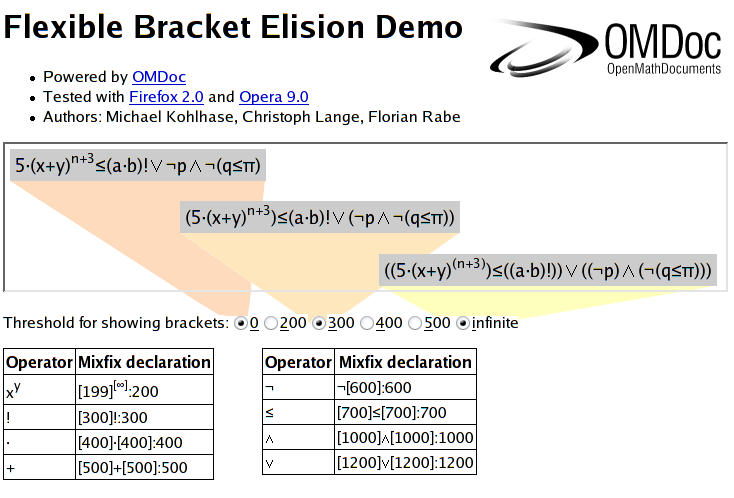
\includegraphics[width=8.5cm]{demo-shot}
    \caption{Flexible Elision of Brackets in XHTML}
    \label{fig:flexible-elision}\vspace*{-.5cm}
\end{figure}
%  \end{wrapfigure}
  We have implemented a prototypical flexible elision scheme for dynamic XHTML, by
  generating tokens for all elidable parts, wrapping them in
  {\element[ns-elt=xhtml]{span}} elements and exporting the elision group and level
  information as XML attributes {\attributeshort[ns-attr=omdoc]{egroup}} and
  {\attributeshort[ns-attr=omdoc]{elevel}} on these elements. All
  {\element[ns-elt=xhtml]{span}} elements with visibility group $g$ and level $l>T_g$ are
  augmented with the attribute {\snippet{style="display:none"}}, which elides them. If the
  user changes the threshold, an embedded {\javascript} function can be used to set the
  display property accordingly. In Figure~\ref{fig:flexible-elision}, we show the system
  with three levels of bracketing thresholds. The same technique would work for
  XHTML+MathML, if the CSS {\tt{display}} directive were implemented for {\mathml}
  elements across browsers. 
\end{newpart}



%%% Local Variables: 
%%% mode: stex
%%% TeX-master: "presel"
%%% fill-column: 90
%%% sentence-end-double-space: nil
%%% End: 

% LocalWords:  FR CL ns elt xhtml attr omdoc egroup elevel stex presel

\newif\ifPDF
\ifx\pdfoutput\undefined\PDFfalse \else\ifnum\pdfoutput >
0\PDFtrue
    \else\PDFfalse
    \fi
\fi

\documentclass[a4paper,11pt,openany,notitlepage]{article}

\title{
\begin{flushright}
Development of an OMGeo Open Markup Format \\ {for the Open GIS Consortium Web Map Service}
\\ {\large{320342 - Guided Research Computer Science -}} \\ {\normalsize{Project Proposal}}
\end{flushright}}
\author{}
\date{}

\usepackage{fancyhdr}
\usepackage{bm}
\usepackage{../../../doc/macros/draftstamp}

\linespread{1.0}

\ifPDF
\usepackage[pdftex]{color,graphicx}
\usepackage[pdftex,bookmarks=true]{hyperref}
\else
\usepackage[dvips]{graphicx}
\usepackage[dvips,bookmarks=true]{hyperref}
\fi

\pagestyle{fancy}
% with this we ensure that the chapter and section
% headings are in lowercase.
%\renewcommand{\chaptermark}[1]{\markboth{#1}{}}
\renewcommand{\sectionmark}[1]{\markright{\thesection\ #1}}
\fancyhf{} % delete current setting for header and footer
\fancyhead[R]{\bfseries\thepage}
\fancyhead[L]{\bfseries\rightmark}
\renewcommand{\headrulewidth}{0.5pt}
\renewcommand{\footrulewidth}{0pt}
\addtolength{\headheight}{2.5pt} % make space for the rule
\addtolength{\textwidth}{1.5cm} \addtolength{\headwidth}{1.5cm}
\addtolength{\topmargin}{-1.0cm} \addtolength{\textheight}{2.2cm}
\addtolength{\hoffset}{-0.5cm}
\fancypagestyle{plain}{%
    \fancyhead{} % get rid of headers on plain pages
    \renewcommand{\headrulewidth}{0pt} % and the line
}

\hypersetup{colorlinks,%
    linkcolor=blue,%
    citecolor=blue,%
    filecolor=blue,%
    urlcolor=blue,%
    bookmarksnumbered,
    bookmarksopen,%
    pdfstartview=FitV,%
    plainpages=false,%
    hypertexnames=false,%
    a4paper}

%%%%%%%%%%%%%%%%%%%%%%%%%%%%%%%%%%%%%%%%%    
\begin{document}

\pagenumbering{roman}
\maketitle \hrule
\begin{flushright}
\Large{\textbf{Alexandru A. Chitea}}
\end{flushright}

\begin{flushright}
\small{a.chitea@iu-bremen.de}
\end{flushright}
\vspace{1cm}
\begin{flushright}
\large{Project Coordinators:}
\end{flushright}

\begin{flushright}
\normalsize{Dr. Peter Baumann - p.baumann@iu-bremen.de}
\end{flushright}
\begin{flushright}
\normalsize{Dr. Michael Kohlhase - m.kohlhase@iu-bremen.de}
\end{flushright}
\vspace{11cm}
International University Bremen\hspace{1.25cm} March 7, 2005\hspace{1.25cm} Spring Semester 2005


\newpage
\tableofcontents
\listoffigures % comment out if you have no figures
\listoftables  % comment out if you have no tables
\pagenumbering{arabic}
\newpage
\section{Executive Summary} \label{sec:execsummary}
\indent

Web Map Services\footnote{The proposed project refers to the Open GIS Consortium WMS Implementation Specification (version 1.1.1) \cite{ogc}.} (WMSes) have been successfully used in a broad range of applications, from meteorology to disaster mitigation. Moreover, as academic and research tools, they are employed by geoscientists to explore discrete properties of the Earth's surface, such as, for example, elevation levels or marine shorelines.

As the WMSes in use today are targeted to specific application areas and cultural backgrounds, their application programming interfaces (APIs) and user-interfaces are therefore hard-coded accordingly. However, most of the times geodata maps need to be exchanged between several clients or manipulated by software applications. A good illustration is the interpretation of two national roadmaps for navigation purposes. For example, when using the German Brandenburg WMS\footnote{The service is restricted to academic use, and hence we cannot provide a valid access URL.}, the term \textit{Strassenorange}\footnote{\textit{Strassenorange} stands for orange street in German.} represents a small road, whereas a French WMS might encode the same data with a different keyword. Therefore the combination of visual representation and the geodata itself leads to conflicts\footnote{E.g.,the language and abbreviated terms may not be international.} between data function and its format, creating bottlenecks in terms of usability.

So far, various schemes for georeferenced data representation have been developed at national scales, but none has yet been adopted as an international standard. The proposed project aims at separating data appearance from its structure through a semantic-based and context-aware technique \cite{mkm2005}. As the OMDoc (\textit{Open Mathematical Documents}) format \cite{kohlhase2004} represents an established method for mathematical knowledge representation and management, we consider extending it to encompass geosemantics. If we succeed in our endeavor, we will achieve a high degree of flexibility in terms of geodata manipulation. Among many others, an envisioned area of application is the disaster mitigation public services\footnote{As major natural cataclysms usually span more than one country, it is of paramount importance to handle in a common way the geodata recorded from multiple WMS providers.}.

%
\section{Summary Description} \label{sec:summarydescr}
\indent

A Web Map Service is an online application that generates maps of georeferenced data. Here, maps are defined to be visual representations of geodata and not the data itself. WMSes employ the digital mapping technique \cite{ogc} to render the geodata in a pictorial format. This approach implies the superimposing of multiple layers that contain georeferenced data, thus allowing map customization through layer addition or removal\footnote{Meteorological services use this feature in a real-time manner to monitor updated information.}.

As it can be seen, the digital mapping technique can be abstracted to a modular concept, where the map layers represent the constituent modules. In this case, a clear division should be established between the functional specifications of the data contained by each layer and the layer's style of representation. Since the OMDoc format successfully achieves this task for mathematical documents, we have envisioned it to be a useful tool for the Web Map Service georeferenced data format, OMGeo. As such, we would like to create an OMDoc extension to encompass the semantics of georeferenced data. Given that OMDoc has been created with a modular concept in mind, an extension to this format implies just the creation of several additional \textit{libraries}\footnote{Here, the term \textit{library} replaces \textit{Content Dictionary} (see Section \ref{subsec:extension}), which is the official OMDoc term.} that will describe the georeferenced data. In addition, a minor extension to the existing OMDoc DTD\footnote{DTD stands for \textit{Document Type Definitions.}} \cite{kohlhasedtd} will be developed to define the additional OMGeo elements.

So far, the user-interfaces of the Web Map Services' application programming interfaces (APIs) are hard-coded at the development stage and geared towards a certain application\footnote{Actually, the language barrier and educational background may also alter the user-WMS interaction.}. Therefore, the interaction with a specific WMS is restricted to a fixed set of clients\footnote{Here, by \textit{clients} we refer to human users or any software application.}. If OMGeo becomes an Open GIS Consortium\footnote{See http://www.opengeospatial.org for more information.} standard for georeferenced data, then clients would be able to create OMGeo documents that could be both human and machine understandable. A direct application of such a document could be the dynamic creation of an API's user-interface to meet a specific user's needs.

%
\section{Research Motivation} \label{sec:motivation}
\indent

In this section, we will address the research motivation behind the development of the OMGeo format in a bottom-up approach. First, we will outline the general capabilities of any Web Map Service\footnote{See the Open GIS Consortium WMS Implementation Specification (version 1.1.1) \cite{ogc}.}. Afterwards, following a description of an ideal client-WMS interaction, the current limitations of the applications using the Web Map Services will be inferred with regard to a real-life example. To conclude this section, we will address the research approach proposed by the project herewith.

\subsection{WMS Capabilities} \label{subsec:capabilities}
\indent

A Web Map Service is an online software system that provides georeferenced data maps. As they were defined earlier (see Section \ref{sec:summarydescr}), maps are the visual representation of geodata and not the data itself. These maps are usually rendered in a pictorial format, and support for different encoding formats\footnote{Most used ones are PNG, GIF and JPEG, and occasionally SVG (Scalable Vector Graphics) or WebCGM (Web Computer Graphics Metafile). \cite{ogc}} is available. Upon requesting a map from a WMS, a client specifies a certain (finite) number of map characteristics. Table \ref{tab:def} outlines these characteristics as they are defined in the Open GIS Consortium WMS Implementation Specification (version 1.1.1) \cite{ogc}.

\begin{table}[h]
	\centering						
		\begin{tabular}{||l|l||} \hline \hline
			\textbf{Map feature}	& \textbf{Description}	\\ \hline \hline
			Layer(s)	& the information to be shown on a map \\ \hline
			Style		& the style associated with each requested	\\
			&	layer	\\ \hline
			Bounding Box		& the portion of the Earth to be mapped;	\\
			& it is axis-parallel \\ \hline
			Spatial Reference System (SRS)		& the projected or geographic coordinate \\
			&	reference system to be used	\\ \hline				
			Output Format		& the pictorial format in which the map	\\
			&	will be rendered	\\ \hline
			Output Size		& the width and height of the output \\
			&	in pixels	\\ \hline
			Background Transparency and Color	& the style of the output's pictorial format \\ \hline \hline
		\end{tabular}
		\caption{Open GIS Consortium WMS Capabilities}		
		\label{tab:def}
\end{table}

\subsection{Client-WMS Interaction} \label{subsec:interaction}
\indent

A standard web browser can ask a Web Map Service to retrieve a map (via a GetMap operation) simply by submitting requests in the form of Uniform Resource Identifiers (URIs) \cite{ogc}. In addition, when retrieving a map, the client can specify, via the WMS user-interface, what and how the information should be shown on the map by selecting different attributes for the parameters described in Table \ref{tab:def}.

Furthermore, the individual map layers can be requested from different Web Map Servers, enabling as such the creation of a network of \textit{distributed map servers} \cite{ogc}. As a direct consequence, a "Cascading Map Server" \cite{ogc} can be established. This would be a WMS that behaves like a client of other WMSes and at the same time behaves like a WMS to other clients. The "Cascading Map Server" approach represents a useful feature as it can perform additional functions such as output format conversion or coordinate transformation on behalf of other servers.

\subsection{Current Limitations} \label{subsec:limitations}
\indent

As it was shown in the previous sections, the Open GIS Consortium WMS Implementation Specification (version 1.1.1) provides the general framework for the behavior of a service that produces georeferenced maps. As such, the standard specifies operations to retrieve a description of the maps offered by a service instance, to retrieve a map, and to query a server about features displayed on a map \cite{ogc}. Therefore, a Web Map Service is implemented with a high degree of usage flexibility. However, limitations, in terms of client-WMS interaction, are induced at the API and presentation levels. Since currently there is no standard to define how geodata should be modeled, many services develop their online applications and model the geodata to meet specific needs. A common approach in this process is to mix the presentation and data representation levels and abstract them to only one level. This level is afterwards hard-coded into both the API, for data retrieval purposes, and the presentation layer. In order to better illustrate this approach, we will refer to the Brandenburg and CubeWerx WMSes\footnote{The two WMSes have been selected as they are conform with the Open GIS Consortium WMS Implementation Specification.} whose user-interfaces can be observed in Figures \ref{fig:cubewerx}\footnote{http://www.cubewerx.com/main/demo$\_$centre.html. Retrieved: March 2, 2005.} and \ref{fig:brandenburg}\footnote{As the service is restricted to academic use only, it cannot be reached at a specific URL. The caption herewith was taken from a local installation.}.
\begin{figure}[h]
	\centering	
		\framebox{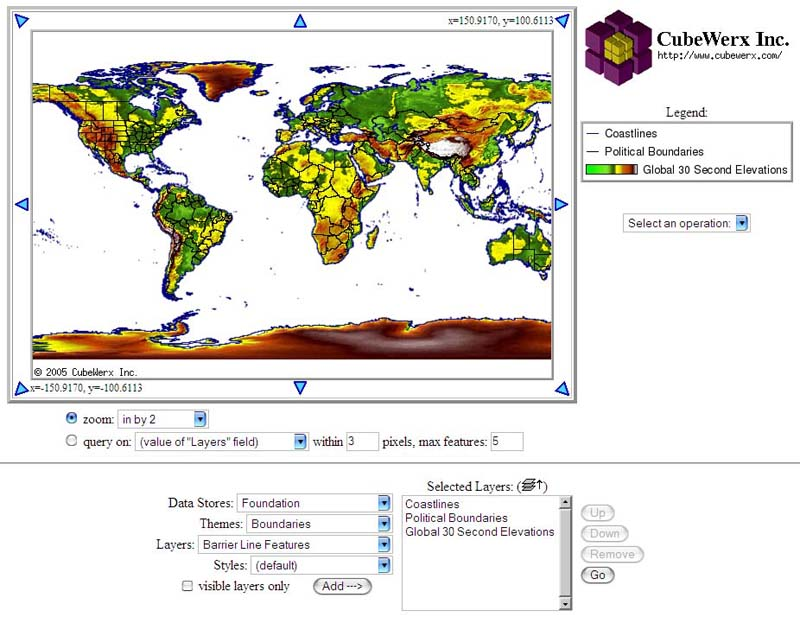
\includegraphics[width=0.90\textwidth]{images/cubewerx.jpg}}
		\caption{CubeXPLOR Demo by CubeWerx Inc.}
	\label{fig:cubewerx}	
\end{figure}
\begin{figure}[h]
		\centering
			\framebox{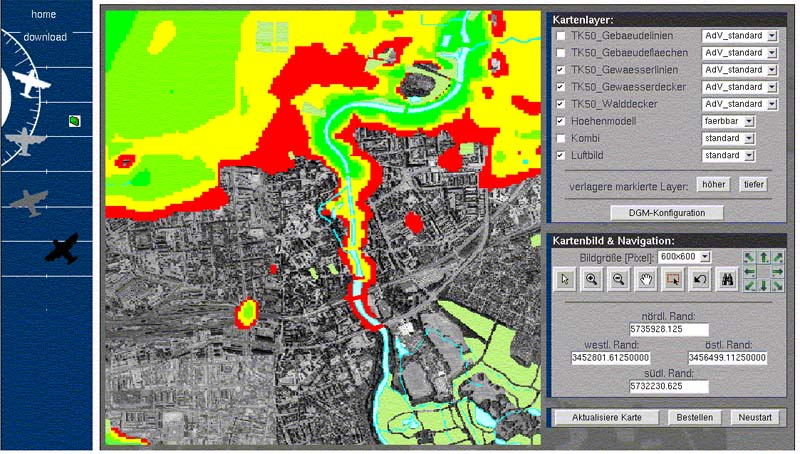
\includegraphics[width=0.90\textwidth]{images/brandenburg.jpg}}
			\caption{Brandenburg WMS - RasGeo Interface}
		\label{fig:brandenburg}
\end{figure}

Even though at their core the two Web Map Services discussed might provide the same capabilities, their user-interfaces and APIs distinguish them in their functionality. Moreover, this functionality is hard-coded and as such these systems cannot dynamically adapt to different user's needs. As it can be observed from Figures \ref{fig:cubewerx} and \ref{fig:brandenburg}, the first noticeable difference is at the language level. Since neither one of the systems provides any description for its terminology and abbreviations, the applications are targeted towards a fixed group of users.

\subsection{Research Approach} \label{subsec:approach}
\indent

As it was shown in Section \ref{subsec:limitations}, the strong interdependence between data representation and its format leads to limitations in terms of application utilities. Since the manipulation of georeferenced data retrieved from various WMSes is of paramount importance in application areas like disaster mitigation, preventing the occurrence of data bottlenecks becomes a top priority.

During the past few years, semantic-based and context-aware techniques have pervaded application areas ranging from science and technology to research and education \cite{mkm2005}. The semantics of an object is determined by its structure (how is the object built up from smaller objects) and its context (what do we already know about these objects, how are they defined, what is their relationship to other objects). As the geodata semantics matches the description above, we have envisioned the development of a knowledge representation and management format, OMGeo, as a solution for separating presentation from structure. However, since we already have an established format for mathematical knowledge, OMDoc, that is both semantic-based and context-aware, we would like to extend it to encompass geosemantics. 

In Section \ref{sec:statement} we will state and analyze the main research problems as they pertain to the development of the OMGeo format, and in Section \ref{sec:strategy} we will detail on the envisioned extension possibility.

%
\section{Statement of the Research Problem} \label{sec:statement}
\indent

As it was shown in the previous sections, the mixture of data format and presentation style considerably reduces the utility of the WMSes. Moreover, since the user-interfaces are hard-coded, clients cannot take full advantage of various WMS applications\footnote{If the user-interface is hard-coded, then the language and the map layers supported are bound to the application in use.} in the absence of nomenclature standards.

Therefore, the overall research problem refers to the separation of the data representation and presentation levels. Furthermore, the data representation level should also encapsulate knowledge about the data in a manner that makes the data content transparent and unambiguous. In the proposed project, we will try to address the following questions:
\begin{enumerate}
	\item Does OMDoc provide a flexible framework to encompass areas of knowledge, other than mathematics?		
	\item Can OMDoc be adapted to encompass geosemantics knowledge?			
	\item How can modularity be achieved so that OMGeo (the extended OMDoc format for georeferenced data) will have an easy way of extending?		
\end{enumerate}

As OMDoc is a semantic-based and context-aware format \cite{kohlhase2004}, we claim that it provides the pillars for the development of OMGeo. Moreover, since the context information for mathematical objects is dynamic and usually both large and highly structured, we assume OMDoc provides a flexible framework to encompass other areas of knowledge \cite{mkm2005}. Since OMDoc was built with a modular concept in mind, extending it involves only the development of additional libraries to capture the geosemantics knowledge. As such, we claim that encompassing geosemantics knowledge can be achieved with minimum adaptation efforts.

As a testing bench for the research claims stated above, the proposed project aims at developing an online demonstrator. In Section \ref{sec:strategy} we will outline the research and development strategy towards the completion of the online demonstrator that will serve as an API to a Web Map Service.

%
\section{Research and Development Strategy} \label{sec:strategy}
\indent

In order to address the research questions and to develop the demonstrator mentioned in Section \ref{sec:statement}, we are planning to carry out the following development steps:
\begin{enumerate}
	\item Extend the OMDoc format to capture geosemantics knowledge.
	\item Develop an OMGeo DTD.
	\item Create sample OMGeo documents.
	\item Develop the API for an example WMS.
\end{enumerate}
The dependence between the above components can be observed in Figure \ref{fig:umlschema}.

Moreover, we will outline each of these components and detail their development process in the next subsections.
\begin{figure}[h]
	\centering		
		\framebox{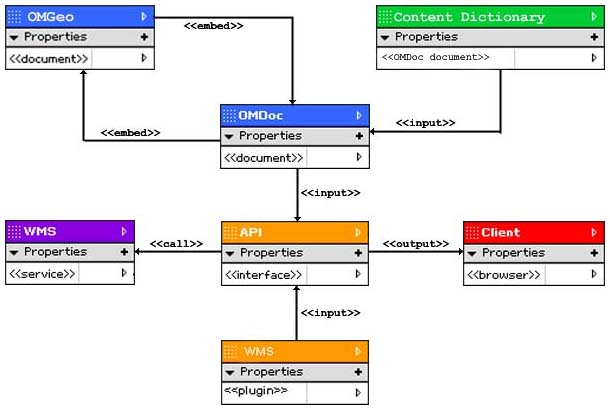
\includegraphics[width=0.90\textwidth]{images/umlschema.jpg}}
		\caption{Module Dependency Schema}
	\label{fig:umlschema}
\end{figure}

\subsection{Extend the OMDoc format to capture geosemantics} \label{subsec:extension}
\indent

As it was shown in the previous sections, a map of georeferenced data can be abstracted to a modular concept with the map layers as the constituent modules. In order to develop a geosemantics format that will overcome the mixture of appearance and structure, we will directly relate to the aforementioned property.

Apart from map data, another area of knowledge where appearance and structure form two distinct entities is mathematics \cite{openmath2004}. The OMDoc format is an open markup language for mathematical documents and more generally the knowledge encapsulated in them in a manner that makes their context and content transparent and unambiguous \cite{kohlhase2004}. It approaches this goal by attaching information to mathematical documents that identify the document structure, the meaning of text fragments, and their relation to other mathematical knowledge in a process called \textit{document markup}. As modular design is generally accepted as best practice in the development of any type of complex application, OMDoc format (version 1.2) also features a modularized language approach. To encompass knowledge, OMDoc makes use of a certain type of libraries called \textit{Content Dictionaries} \cite{kohlhase2004}. A Content Dictionary acts as a container for sets of symbol declarations and knowledge about them, and marks them by \textbf{theory} elements. As such, the OMDoc format becomes easily extensible since the provision of knowledge through Content Dictionaries can make the format applicable to other areas, apart from mathematics. Therefore, in order to encapsulate geodata knowledge, the proposed project aims at developing a number of Content Dictionaries that will refer to the different constituent blocks of a map.

As the content of the \textit{Content Dictionaries} is highly specialized, this project will require a transdisciplinary approach with input from the geoscience field. In order to achieve a better design and better content information, we will cooperate with Prof. Dr. Vikram Unitham from International University Bremen.

\subsection{Develop an OMGeo DTD} \label{subsec:dtd}
\indent

As it was shown in subsection \ref{subsec:extension}, the proposed project aims at developing an extension to OMDoc to include geosemantics knowledge. In order to specify how the geodata should be encapsulated in an OMDoc document, a DTD extension should be attached to the present OMDoc DTD. Even though the RelaxNG\footnote{See http://www.relaxng.org for more information.} method is slowly replacing the DTD and Schema specifications, an OMGeo DTD extension will still be provided. The elements to be defined by the DTD are as yet to be clarified, and will be one of the project results.

\subsection{Create sample OMGeo documents} \label{subsec:sample}
\indent

Upon the creation of valid Content Dictionaries that encapsulate geodata knowledge, documents of OMGeo papers can be written. A case study on sample OMGeo documents will be conducted to test the format's capabilities. Moreover, these documents will also be used as an input to the online demonstrator.

\subsection{Develop the API for an example WMS} \label{subsec:demonstrator}
\indent

Having set up the basis to develop OMGeo documents that are both human and machine understandable, the proposed project will be concluded with an online demonstration of how these documents can interact with a given Web Map Service. For this purpose, an application programming interface will be developed. This API will be developed using J2EE\footnote{See Section \ref{sec:development} for further explanations.} technology and will basically perform the following tasks:
\begin{enumerate}
	\item Receive a plugin\footnote{The plugin will be an XML file where the OMGeo elements will be mapped to WMS specific keywords that are used to query the database.} that will contain the definitions for a specific Web Map Service.
	\item Receive an OMGeo document.
	\item Dynamically transform the OMGeo document into a user-interface.
	\item Use the knowledge encapsulated in the OMGeo document to query the WMS database.
	\item Display the requested map from the Web Map Service.
\end{enumerate}
The module dependency schema in Figure \ref{fig:umlschema} provides a visual representation of the above modules.

%
\section{Development Framework} \label{sec:development}
\indent

As the proposed project considers the development of an online demonstrator as a testing bench, we will outline in this section the software development framework. In particular, we will address the environment and tools that will be used throughout the project. As a conclusion of the section, a reference guide to the expected results will be proposed.

\subsection{Environment and Tools} \label{subsec:tools}
\indent

As the development of the online demonstrator involves querying a Web Map Service, we will make use of the Brandenburg WMS. Since this service is restricted to academic use, it is not publicly available at a specific URL. Therefore, we will make a local installation on a CLAMV\footnote{\textit{CLAMV} stands for \textit{Computational Laboratory for Analysis, Modeling, and Visualization}. More info at http://www.clamv.iu-bremen.de} station. As such a PostgreSQL\footnote{See http://www.postgresql.org for more information.}/Rasdaman\footnote{See http://www.rasdaman.com for more information.} database will be installed on top of a Tomcat server. For the API development, we will use the Java 2 Platform, Enterprise Edition\footnote{J2EE defines the standard for developing component-based multitier enterprise application, featuring Web services support and development tools.} (J2EE). In particular, we will use the Java servlets and Java Server Pages (JSP) technologies. Since the software application will be developed under Linux, we will configure the Emacs editor as a Java IDE (Integrated Development Environment) by installing the Java Development Environment (JDE) for Emacs\footnote{See http://www-106.ibm.com/developerworks/library/j-emacs/?n-j-5241 for more information.}.

\subsection{Expected Results} \label{subsec:results}
\indent

As a suitable evaluation criterion, we would define this project to be successful upon the completion of a running version of the online demonstrator. Since this software application relies on several input modules, we regard the completion of the plugin for the Brandenburg WMS and the creation of the Content Dictionaries for the geosemantics knowledge as important milestones in the overall development. However, as the geosemantics standard behind a georeferenced map does not exist in a unified model, we will not regard our Content Dictionaries to be exhaustive. In the following sections, we will briefly outline a timeline for the proposed project.

%
\section{Schedule of Activities} \label{sec:schedule}
\indent

The activities listed below relate to the Gantt chart in Figure \ref{fig:timeline} that briefly outlines a timeline for the proposed project.
\begin{enumerate}
	\item Develop OMDoc Content Dictionaries to capture geosemantics knowledge.
	\item Develop the OMGeo DTD as an extension of the OMDoc DTD.
	\item Create sample OMGeo documents.
	\item Develop the API WMS plugin for the Brandenburg WMS.
	\item Develop the API for the Brandenburg WMS.
	\item Develop the website that will incorporate the API.
	\item Conduct testing sessions on sample OMGeo documents.
\end{enumerate}
\begin{figure}[h]
	\centering		
		\framebox{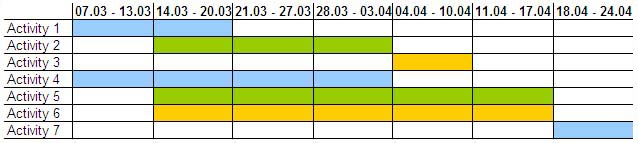
\includegraphics[width=0.90\textwidth]{images/timeline.jpg}}
		\caption{Schedule of Activities}
	\label{fig:timeline}
\end{figure}

Moreover, we will provide a Final Report of the proposed project on April 25, 2005 and will orally present our results in the beginning of May 2005 at International University Bremen.
%
\newpage
%%%%%%%%%%%%%%%%%%%%%%%%%%%%%%%%%%%%%%%%%%%%%%%%%%%%%%%%%%%%%%%%%%
%                                                                %
%                                                                %
%                     The Bibliography                           %
%                                                                %
%                                                                %
%%%%%%%%%%%%%%%%%%%%%%%%%%%%%%%%%%%%%%%%%%%%%%%%%%%%%%%%%%%%%%%%%%

\begin{thebibliography}{0}
%
\bibitem{kohlhase2004}
Kohlhase, M. (2004). OMDoc - An Open Markup Format for Mathematical 
Documents (version 1.2) \textit{http://www.mathweb.org/omdoc/omdoc.ps}, manuscript.
%
\bibitem{kohlhasedtd}
Kohlhase, M. (2004). The OMDoc Document Type Definition \textit{http://www.mathweb.org/omdoc/dtd/omdoc.dtd}.
%
\bibitem{ogc}
de la Beaujardiere, J. (2002). Web Map Service Implementation Specification (version 1.1.1) \textit{Open GIS Consortium Implementation Specification}.
%
\bibitem{openmath2004}
Buswell, S. Caprotti, O. Carlisle, D.P. Dewar, M.C. Gaetano, M. Kohlhase, M. (2004). The OpenMath Standard (version 2.0) \textit{The OpenMath Society}.
%
\bibitem{mkm2005}
Kohlhase, M. (2005). Mathematical Knowledge Management Network of Excellence (version 2.0) \textit{Proposal draft}.
%
\end{thebibliography}

\end{document}

\svnInfo $Id: compatibility.tex 6837 2007-09-23 00:07:39Z frabe $
\svnKeyword $HeadURL: https://svn.omdoc.org/repos/omdoc/projects/omdoc-2.0/OpenMath-paper/compatibility.tex $
\section{Compatibility}\label{sec:templates}
Here we show that the proposed infrastructure for notation definitions is a superset of
the functionality of other systems. We first show that we can re-gain the {\omdocv{1.2}}
syntax by specifying two new elements that get their meaning as abbreviations of the new
functionality. In a second step we develop a template-based variant of our presentation
technique to be compatible to (a functional superset of) the {\activemath} notation
definition system. 

\subsection{Compatibility to {\omdocv{1.2}}}

The proposed presentation syntax has one disadvantage: Information about the fixity or
associativity of a symbol is not marked up explicitly. Therefore, we specify
{\element{use}} elements in the next section which are very similar to the corresponding
{\omdocv{1.2}} syntax.

The {\element{style}}- and {\element{xslt}}-based infrastructure for notation definitions
in {\omdocv{1.2}} will not be supported. They have rightfully been described as
non-declarative, therefore ill-suited as a definitional mechanism and have tied the
presentation procedure to the XSLT programming language. The extended expressivity of the
proposed notation definition format seems to cover all the cases, where these two have
been needed in practice. We have re-formulated\ednote{MK: complete this} all the notation
definitions in the {\openmath} standard content dictionaries --- which cover the K-14
fragment of mathematics --- and have not found need for a procedural fall-back solution.


\subsection{Direct Specification of Symbol Characteristics}

We define a presentation element {\element{use}} which like its counterpart in
{\omdocv{1.2}} is based on the direct specification of symbol characteristics. But here we
define its meaning via abbreviations for certain presentations in the above syntax.
\begin{center}\small
\begin{tabular}{|l|l|p{3.2cm}|p{3.5cm}|}\hline
  Element  &  \multicolumn{2}{c|}{Attributes}  &  Content \\\cline{2-3}
  & Required & Optional & \\\hline\hline
  use           &          & egroup, elevel, precedence, bracket-style, fixity
                     & rbrack? lbrack? operator? separator?\\\hline
  operator      &          & egroup, elevel             & \llquote{item}* \\\hline\hline
  lbrack        &          & egroup, elevel             & \llquote{item}* \\\hline
  rbrack        &          & egroup, elevel             & \llquote{item}* \\\hline
  \multicolumn{4}{|l|}{\llquote{item} $\hat=$ (text $|$ element $|$ map $|$ attribution $|$
recurse)}\\\hline
\end{tabular}
\end{center}

A {\element{use}} may have the attributes
\begin{itemize}
\item {\attribute{fixity}{use}} with values {\attval{prefix}{fixity}{use}},
  {\attval{postfix}{fixity}{use}}, {\attval{infixl}{fixity}{use}},
  {\attval{infixr}{fixity}{use}}, and {\attval{infixlr}{fixity}{use}},
\item If fixity is {\attval{prefix}{fixity}{use}} or {\attval{postfix}{fixity}{use}}:
  {\attribute{bracket-style}{use}} with values {\attval{math}{bracket-style}{use}} and
  {\attval{lisp}{bracket-style}{use}}\ednote{discuss that! --CL},
  % \item optionally, {\attribute{crossref-symbol}{use}} whose value must be a
  %   whitespace-separated list of {\attval{lbrack}{crossref-symbol}{use}},
  %   {\attval{rbrack}{crossref-symbol}{use}}, and
  %   {\attval{separator}{crossref-symbol}{use}} with default value being the empty
  %   string.
\item {\attribute{precedence}{use}}.
\end{itemize}
Its children are at most one each of {\element{lbrack}}, {\element{rbrack}},
{\element{operator}}, and {\element{separator}}, all with \llquote{item}* content.
\ednote{FR: This should be improved: It should be possible that a use element gives only, e.g., fixity and precedence with the rest being inherited from default presentations. The motivation is that fixity and precedence typically depend on the symbol but not on the output format, whereas the other attributes typically depend on the home theory and the output format.}
Such a presentation specification can be translated easily into the above syntax. For
prefix operators,

\begin{minipage}{.53\textwidth}
\begin{lstlisting}[mathescape,frame=tlrb,numbers=none]
<use fixity="prefix" bracket-style="math" precedence="$p$">
  <lbrack>$\llquote{l}$</lbrack>
  <rbrack>$\llquote{r}$</rbrack>
  <operator>$\llquote{op}$</operator>
  <separator>$\llquote{s}$</separator>
</use>
\end{lstlisting}
\end{minipage}
\quad abbreviates\quad
\begin{minipage}{.28\textwidth}
\begin{lstlisting}[mathescape,frame=tlrb,numbers=none]
$\llquote{op}$
$\llquote{l}$
<map begin="1" end="-1">
  <separator>$\llquote{s}$</separator>
  <recurse precedence="$p$"/>
</map>
$\llquote{r}$
\end{lstlisting}
\end{minipage}

And

\begin{minipage}{.53\textwidth}
\begin{lstlisting}[mathescape,frame=tlrb,numbers=none]
<use fixity="prefix" bracket-style="lisp" precedence="$p$">
  <lbrack>$\llquote{l}$</lbrack>
  <rbrack>$\llquote{r}$</rbrack>
  <operator>$\llquote{op}$</operator>
  <separator>$\llquote{s}$</separator>
</use>
\end{lstlisting}
\end{minipage}
\quad abbreviates\quad
\begin{minipage}{.28\textwidth}
\begin{lstlisting}[mathescape,frame=tlrb,numbers=none]
$\llquote{l}^b$
$\llquote{op}$
$\llquote{s}$
<map begin="1" end="-1">
  <separator>$\llquote{s}$</separator>
  <recurse precedence="$p$"/>
</map>
$\llquote{r}^b$
\end{lstlisting}
\end{minipage}
where the superscript $b$ denotes that the attribute \snippet{level="bracket"}
has been added to the elements $l$ and $r$. Note how in the mathematical bracket
style brackets are always displayed, whereas they can be elided in the Lisp
style\ednote{@FR: Not in general! For postfix (e.\,g.\ factorial) and infix (most
  ordinary operators), yes, but for prefix? --CL}. Postfix operators are treated
correspondingly.

If omitted {\element{lbrack}}, {\element{rbrack}}, and {\element{separator}} default to
the empty elements\ednote{I thought in OMDoc 1.2 they defaulted to ( and )? --CL}, and
{\element{operator}} defaults to \snippet{map begin="0"/>}. {\attribute{fixity}{use}}
defaults to {\attval{prefix}{fixity}{use}}, {\attribute{bracket-style}{use}} to
{\attval{math}{bracket-style}{use}}, and {\attribute{precedence}{use}} to
{\attval{0}{precedence}{use}}.

% Here, and in the following, $C$ abbreviates \snippet{crossref="true"} if the
% corresponding element is in the value of \attribute{crossref-symbol}{use}, and is empty
% otherwise.

Infix operators require some care: An infix operator which is applied to $n$ arguments is
inserted $n-1$ times between the arguments. {\attval{infixlr}{fixity}{use}} is used for
associative operators for which no inner brackets are needed.
{\attval{infixl}{fixity}{use}} and {\attval{infixr}{fixity}{use}} refer to left and
right-associative operators, respectively. In none of these cases do we generate inner
brackets, not even elidable ones. This permits us to distinguish, e.\,g., the $n$-ary
application of addition from successive application of binary addition.

Elidable or unelidable brackets are only generated when the several applications of the
operator are nested. This is achieved by different input precedences when
expanding. Associative, right-associative, and left-associative infix specifications
expand to, respectively,
\begin{center}
\begin{minipage}{.3\textwidth}
\begin{lstlisting}[mathescape,frame=tlrb,numbers=none]
$\llquote{l}^b$
<map begin="1" end="-1">
  <separator>$\llquote{op}$</separator>
  <recurse precedence="$p$"/>
</map>
$\llquote{r}^b$
\end{lstlisting}
\end{minipage}
\quad
\begin{minipage}{.3\textwidth}
\begin{lstlisting}[mathescape,frame=tlrb,numbers=none]
$\llquote{l}^b$
<map begin="1">
  <separator/>
  <recurse precedence="$p-1$"/>
</map>
<map begin="2" end="-1">
  <separator/>
  $\llquote{op}$
  <recurse precedence="$p$"/>
</map>
$\llquote{r}^b$
\end{lstlisting}
\end{minipage}
\quad
\begin{minipage}{.3\textwidth}
\begin{lstlisting}[mathescape,frame=tlrb,numbers=none]
$\llquote{l}^b$
<map begin="1" end="-2">
  <separator/>
  <recurse precedence="$p$"/>
  $\llquote{op}$
</map>
<map begin="-1">
  <separator/>
  <recurse precedence="$p-1$"/>
</map>
$\llquote{r}^b$
\end{lstlisting}
\end{minipage}
\end{center}

\subsection{Compatibility to {\activemath}}

  The {\activemath} system~\cite{URL:activemath} uses a pattern-based approach that
  synthesizes ideas from the {\omdocv{1.0}} infrastructure and~\cite{Naylor:conversion}
  for XSLT template generation.
\begin{lstlisting} 
<symbolpresentation xmlns="..." id="comb1bk" xref=".../bk">
  <notation format="html|pmathml|TeX" language="de">
    <math xmlns="http://www.w3.org/1998/Math/MathML">
      <mrow><mo>(</mo><mfrac linethickness="0"><mi>n</mi><mi>k</mi></mfrac><mo>)</mo></mrow> 
    </math>
    <OMOBJ xmlns="http://www.openmath.org/OpenMath">
      <OMA><OMS cd="comb1" name="bk"/><OMV name="n"><OMV name="k"></OMA>
    </OMOBJ>
  </notation>
</symbolpresentation>
\end{lstlisting}
  The presentation approach outlined in~\cite{ManLib:apo05} directly uses the names of
  {\openmath} variables and the content of {\mathml} {\element{mi}} elements for the
  necessary cross-referencing between formats, confusing the role of meta-variables and
  object variables. Conceptually, this is a step backwards from~\cite{Naylor:conversion}
  (where the distinction was somewhat tentative) and makes it impossible to exclude
  variables from the cross-referencing (and therefore recursion) of the presentation
  procedure. The main contribution here is the provision of the
  {\textit{jEditOQMath}}~\cite{jeditoqmath:web} developed by P.\
  Libbrecht~\cite{Lib:authoring} with a {\openmath} Presentation Editor (OMPE)
  plug-in~\cite{oqmath:web} for the visual authoring of {\element{symbolpresentation}}
  elements.

\begin{newpart}{MK: we have to talk about this}
  \subsection{A Pattern-Based Approach to Flexary Mixfix Notations}

%\begin{newpart}{FR: pattern example for mathml draft}
%\documentclass{article}
\usepackage{listings,ed}
\usepackage{lstomdoc}

\begin{document}

Idea of semantics: A substitution component is given by arglist/.../arglist/arg and accessed by iterate/.../iterate/render with corresponding names. The substitution component at the current position in the match of arglist/.../arglist/arglist is accessed by iterate/.../iterate/render, too. If a render cannot be resolved, the name of its iterate parent is prepended.

Flexary bounded integral as non-atomic binder presented by using nested patterns

\ednote{I use Latex because I don't know MathML.}
\ednote{I don't use the official symbol and theory names because I don't know them.}

\begin{lstlisting}
<presentation format="latex">
  <prototype>
    <OMBIND>
      <OMA>
        <OMS name="int"/>
        <arglist name="domains">
          <OMA>
            <OMS name="interval"/>
            <arg name="lower_bound"/>
            <arg name="upper_bound"/>
          </OMA>
        </arglist>
      </OMA>
      <OMBVAR>
        <arglist name="variables"/>
      </OMBVAR>
      <arg name="condition"/>
      <arg name="body"/>
    </OMBIND>
  </prototype>
  <rendering>
    <text>\mathop{</text>
    <iterate name="domains">
      <separator><text> </text></separator>
      <text>\int_{</text>
      <render name="lower_bound"/>
      <text>}^{</text>
      <render name="upper_bound"/>
      <text>}</text>
    </iterate>
    <text>}_{</text>
    <render name="condition"/>
    <text>}</text>
    <render name="body"/>
    <iterate name="variables" reverse="Yes">
      <text>d <text>
      <render name="variables"/>
    </iterate>
\end{lstlisting}

Intended presentation of \[\beta(@(int,interval(a_1,b_1),interval(a_2,b_2)),x_1,x_2,@(>,x_1,x_2),@(f,x_1,x_2))\] is
\[\mathop{\int_{a_1}^{b_1}\int_{a_2}^{b_2}}_{x_1>x_2}f(x_1,x_2)d x_2 d x_1\]

Note: This does not work for a flexary integral where set and interval bounds are mixed.

Note: This does not work if the bound variables have attributions. (The same problems occurs for the pattern that matches a lambda binder that is already used in the specification.)
\end{document}

%\end{newpart}


  Template-based approaches are often simpler to understand for authors, moreover, they
  are the only intuitive way to capture notations like $\sin^2(x)$ for the square of the
  value of the sine function at $x$. Here we propose to directly follow the lead of the
  Naylor\&Watt system described in Section~\ref{sec:notdef}, re-using as much of the
  infrastructure we have built up until now as possible. Furthermore, we will drop the
  distinction between a semantic template and the notation generators. We claim that
  template-based notation definitions should only contain information about
  ``corresponding'' representations, and that presentation generation is only one
  direction of transformation between representations (from machine-oriented to
  human-oriented ones). The the symmetricity of the ``correspondence relation'' is
  immediately perspicuous if we have templates for more than one machine-oriented format,
  e.\,g.\ {\openmath} and content {\mathml}. But parsing of human-oriented formats should in
  principle be able to use the information in the ``notation correpsondence'' in the
  opposite of the ``presentation direction''. We should be able to derive parsing-oriented
  grammars taking into account precedences and the extended elision specifications
  developed above. In this paper though, we will not make use of this generalization and
  only concentrate on the presentation direction. Concretely, we assume that the
  presentation algorithm either directly uses the {\openmath} template for pattern
  matching internally, or generates XPath expression for the
  {\attribute[ns-elt=xsl]{match}{template}} attribute in the {\element[ns-elt=xsl]{template}}
  element as in {\mylstref{template}}.


  Finally, we keep the set of corresponding templates loosely coupled, rather than enging
  them in a {\element{Notation}} element as in {\mylstref{lst:template-based}}: Two
  {\element{presentation}} elements are in correspondence, if they reference the same
  symbol in the {\attribute{for}{presentation}} element and have the same
  {\attribute{role}{presentation}} value.

  Consider for instance the case of the typing judgment from {\mylstref{typing-judgment}},
  here we would just add the following template. 
\begin{lstlisting}[mathescape]
<presentation format="OM" for="#typing-judgment">
  <OMA><OMS cd="types" name="typing-judgment"/>
    <arg name="context"/><arg name="sig"/><arg name="term"/><arg name="type"/>
  </OMA>
</presentation>
\end{lstlisting}
  Unfortunately, we cannot directly write this in our grammar (nor would we like allow
  this, since we want to support an open-ended set of XML-based formats). Therefore we
  write instead
\begin{lstlisting}[mathescape]
<presentation format="OM" role="application" for="#typing-judgment">
  <element name="OMA">
    <element name="OMS">
      <attribute name="cd"><text>types</text></attribute>
      <attribute name="name"><text>typing-judgment</text></attribute>
    </element>
    <arg name="context"/><arg name="sig"/><map name="term"/><map name="type"/>
  </element>
</presentation>
\end{lstlisting}
  This template is assembled using the {\omdoc} {\element{element}} and
  {\element{attribute}} elements, rather than the {\openmath} elements themselves. We
  consider this representation above to be equivalent to the one that uses the target
  elements literally.

  Following XSLT terminology, we call we speak of the {\defemph{native}} encoding for the
  former representation and the {\defemph{literal inclusion}} encoding for the
  latter. Note that the native encoding has great advantages for validation, while the
  literal inclusion encoding is simpler to read for humans. They are obviously identical
  in expressivity and trivially isomorphic. We therefore assume that native form is used
  for storage and a pre-process or a tool like OMPE will present equivalent literal
  inclusion syntax for editing and user interaction. In particular, we will write our
  examples in literal inclusion encoding.

  \begin{newpart}{@MK: I only understood this stuff when you gave the additional PMML
      pattern and told me that one way of the presentation could be ``pattern matching
      OM'' $\to$ ``output PMML''. Therefore, I want an PMML example here and an
      explanation; please adapt this draft. --CL}
\begin{lstlisting}[mathescape]
<presentation format="pmathml" for="#typing-judgment">
  <mrow>
    <arg name="context"/>
    <msub><mo>$\vdash$</mo><arg name="sig"/></msub>
    <arg name="term"/>
    <mo>:</mo>
    <arg name="type"/>
  </mrow>
</presentation>
\end{lstlisting}
    
    When for the same symbol there is a presentation pattern $p_{in}$ for the given input
    format (e.\,g.\ {\openmath}) and $p_{out}$ for the desired output format (e.\,g.\
    Presentation {\mathml}), the input would be matched against $p_{in}$, assigning the
    meta-variables named by the {\attribute{name}{map}} attribute. Then, the output would
    be rendered according to $p_{out}$, filling in the results of recursively rendering
    the values of the meta-variables at the indicated positions.
  \end{newpart}

  Note that the native encoding also clarifies the role of the {\element{map}} elements as
  meta-variables, and the contribution of the other presentation elements.

\begin{lstlisting}[mathescape]
<presentation for="#plus" role="constant" format="OM"><OMS cd="arith1" name="plus"/></presentation>
<presentation for="#plus" role="application" format="OM">
  <OMA><OMS cd="arith1" name="plus"/><map begin="1" end="-1" name="summands"/></OMA>
</presentation>
<presentation for="#plus" role="application" format="ascii latex">
  <element name="mo" egroup="lbrack"><text>(</text></element>
  <map name="summands"><separator><arg pos="0"/></separator><recurse/></map>
  <element name="mo" egroup="lbrack"><text>(</text></element>
</presentation>
\end{lstlisting}
  \ednote{MK: say something about the referencing with @name and @begin/end/pos, and where
    what is redundant. But @name is always a good documentation of the intended behavior.}
\end{newpart}




%%% Local Variables: 
%%% mode: stex
%%% TeX-master: "presel"
%%% fill-column: 90
%%% sentence-end-double-space: nil
%%% End: 


% LocalWords:  CL rbrack lbrack infixl infixr infixlr crossref whitespece tlrb
% LocalWords:  mathescape FR OMDoc assoc ary op ednote symbolpresentation xmlns
% LocalWords:  bk xref html pmathml de mrow mo mfrac linethickness mi OMOBJ OMA
% LocalWords:  OMS cd OMV MK jEditOQMath OMPE Vorher hieß es noch Das hier ist
% LocalWords:  doch nicht Warum denn auf einmal Ausgabeformat OM Im ersten bzw
% LocalWords:  Beispiel wenn wir von sprechen wollen wäre MathML sinnvoll aber
% LocalWords:  eine Identitäts Abbildung Außerdem geht ein der Eingabesprache
% LocalWords:  macht das und Ausgabesprache PMML nimmt gematchten Ausdrücke pre
% LocalWords:  crid arith stex presel egroup elevel

\svnInfo $Id: outlook.tex 6570 2007-06-27 08:40:11Z clange $
\svnKeyword $HeadURL: https://svn.omdoc.org/repos/omdoc/projects/omdoc-2.0/OpenMath-paper/outlook.tex $
\section{Conclusion and Outlook}\label{sec:outlook}

The advantage of content-oriented representation formats for mathematical formulae is that
they are independent or a specific output format, and that human-oriented presentations
can be generated taking into account user preferences, device constraints, etc. To realize
this potential, we need presentation algorithms that are
\begin{description}
\item[knowledge-based] The knowledge about notations and their use is an integral part of
  our mathematical expertise. If a presentation algorithm is not, then it becomes
  unmaintainable.
\item[extensible] Just as mathematics itself, mathematical notation is never finished; new
  notations are always invented, and they are introduced and discarded on the fly.
\item[adaptive] They should allow to take the user's preferences into account. In the end,
  the purpose of mathematical notation is to support a reader in understanding mathematics
  as effortlessly as possible --- and people differ in their cognitive styles.
\item[mathematical] They should be able to model as many mathematical practices as
  possible, so that mathematicians are not hindered by system restrictions in the
  available notations.
\item[efficient] Presentation generation should not bog down servers, and should run on
  all kinds of clients with little lag. The time of the working mathematician is precious!
\end{description}
The first three of these aspects call for an meta-mathematical language for
{\emph{notation definitions}} which can be managed by MKM tools. A corollary of the
manageability postulate is that the notation definition language should be
{\emph{declarative}}. 

In this paper, we have presented an infrastructure for declarative notation definitions
building on ideas from {\omdocv{1.2}} and the presentation system of the {\isabelle}
theorem prover. We have incorporated functionality for flexary applications and binders
necessary to apply these ideas to {\openmath} and content {\mathml}, and we have extended
the {\isabelle}'s precedence-based elision algorithm with general flexible elision
functionality, which covers most mathematical elision practices. We conjecture that
others, like Church's dot notation can be specified by allowing more values for the
{\attributeshort{egroup}} attribute.

Actually, the dot notation is a representative of a more general, user-adaptive practice
that we do not cover in this paper: {\emph{abbreviation}}. If a formula is too large or
complex to be digested in one go, mathematicians often help their audience by abbreviating
parts, which are explained in isolation or expanded when the general picture has been
grasped. We feel that the abbreviation generation problem shares many aspects with
elisions, but is less structured, and more dependent on modeling the abilities and
cognitive load of the reader. Therefore we expect the elision techniques presented in this
paper to constitute a first step into the right direction, but also that we need more
insights to solve the abbreviation generation problem.

Another problem we have not addressed in this paper even though it is very related is the
problem of reversing generation in the parsing process for mathematical formulae\ednote{I
  guess we did in the compatibility section. --CL}: In some situations, the symbol
characteristics are sufficient to allow a mathematical software system to reconstruct the
content structure from its presentation. In the case of the {\isabelle} system, this
property is essential to ensure unambiguous input. In this paper, we will not pursue the
question of parseability, since the flexible elision of arguments is not sufficiently
understood to warrant a restriction to an invertible presentation process. In fact, we
have argued elsewhere\cite{Kohlhase04:stex} that the process of parsing mathematical
formula is AI-hard\footnote{i.e. we cannot solve the problem short of succeeding at
  Artificial Intelligence} in the worst case, since it pre-supposes a mathematical
understanding of the communicated concepts.

We have implemented the approach presented in this paper in a Scala class\ednote{@CL/FR:
  cite, is that correct?} to evaluate the expressivity and efficiency of our approach.
First results are very promising; we will release the finished implementation under an
open source license as a basis for practical presentation systems.

After a thorough evaluation we want to incorporate the presentation infrastructure
presented in this paper into the {\omdocv{2.0}} format currently under development, and we
propose it as part of the content dictionary mechanism of the upcoming {\mathml}3
recommendation.

%%% Local Variables: 
%%% mode: stex
%%% TeX-master: "presel"
%%% fill-column: 90
%%% sentence-end-double-space: nil
%%% End: 

% LocalWords:  egroup Scala CL FR presel

\bibliography{kwarc} 
\bibliographystyle{alpha}
\svnInfo $Id: appendix.tex 6573 2007-06-27 14:25:23Z kohlhase $
\svnKeyword $HeadURL: https://svn.omdoc.org/repos/omdoc/projects/omdoc-2.0/OpenMath-paper/appendix.tex $
\begin{appendix}
  \section{A first RelaxNG Grammar}
  \lstinputlisting[language=RNC,nolol,frame=none]{pres.rnc}
  \section{Complex Examples}

  \lstinputlisting{newint.om}
  \lstinputlisting{newint.pres}
  makes ${\int_{S1}\int_{S2}\int_{S2}\atop x_1>1\wedge x_2>1\wedge x_3>1} x_1+2x_2^2+3x_3^3
  dx_3dx_2 dx_1$
\end{appendix}


%%% Local Variables: 
%%% mode: stex
%%% TeX-master: "presel"
%%% End: 

% LocalWords:  RelaxNG RNC nolol pres rnc stex presel

\end{document}

%%% Local Variables: 
%%% mode: latex
%%% TeX-master: t
%%% fill-column: 90
%%% sentence-end-double-space: nil
%%% End: 

% LocalWords:  kwarc
